\documentclass{beamer}

\usepackage[utf8]{inputenc}
\usepackage[T2A]{fontenc}
\usepackage[russian]{babel}

\usefonttheme{serif}

\usepackage{amsmath}
\usepackage{amssymb}
\usepackage{amsthm}
\usepackage{amsfonts}
\usepackage{braket}
\usepackage{color}
\usepackage{graphicx}
\usepackage{textpos}

\newcommand{\pdfimg}[2]{\newline\centerline{\includegraphics[width=#2]{#1}}\newline}

\definecolor{myred}{rgb}{0.75, 0.0, 0.0}
\definecolor{mygreen}{rgb}{0.0, 0.5, 0.1}
\newcommand{\rc}[1]{\textcolor{myred}{#1}}
\newcommand{\gc}[1]{\textcolor{mygreen}{#1}}
\newcommand{\bc}[1]{\textcolor{blue}{#1}}

\begin{document}

\title{Квантовые вычисления}
\subtitle{
	Основные принципы.\newline
	Примеры квантовых алгоритмов.\newline
	Сложности реализации.\newline
	Недавние достижения.
}
\date{}

\frame{\titlepage} 

\section{Основы}
\frame{
	\frametitle{Кубит}
	$$\ket{\theta} = \alpha\ket{0} + \beta\ket{1}$$
	$$\alpha, \beta \in \mathbb{C};\; |\alpha|^2 + |\beta|^2 = 1$$
	\pause
	$$\ket{\phi} = \rc{\alpha_\phi} \ket{0} + \rc{\beta_\phi} \ket{1}$$
	$$\ket{\psi} = \bc{\alpha_\psi} \ket{0} + \bc{\beta_\psi} \ket{1}$$
	$$\ket{\phi\psi} = \rc{\alpha_\phi} \bc{\alpha_\psi} \ket{00} + \rc{\alpha_\phi} \bc{\beta_\psi} \ket{01} + 
	  \rc{\beta_\phi} \bc{\alpha_\psi} \ket{10} + \rc{\beta_\phi} \bc{\beta_\psi} \ket{11}$$
	\pause
	$$\ket{\phi\psi} = a \ket{00} + b \ket{01} + c \ket{10} + d \ket{11}, bc = ad$$
	\pause
	$$\ket{\nu_1 \nu_2 ... \nu_n} = \sum_{i=0}^{2^n - 1}{\alpha_i \ket{i}}, \; \sum_{i={0}}^{2^n - 1}{|\alpha_i|^2} = 1$$
}

\frame{
	\frametitle{Квантовые вентили}
	\pause
	$$\hat{U}_{not}\ket{0} = \ket{1},\; \hat{U}_{not}\ket{1} = \ket{0}$$
	\pause
	$$\hat{H}\ket{0} = \frac{\ket{0} + \ket{1}}{\sqrt{2}},\; \hat{H}\ket{1} = \frac{\ket{0} - \ket{1}}{\sqrt{2}}$$
	\pause
	$$\hat{R}(\theta)\ket{0} = \ket{0},\; \hat{R}(\theta)\ket{1} = e^{2\pi i\theta}\ket{1}$$
	\pause
	$$\hat{U}_{cnot}\ket{a,b} = \ket{a, a + b}$$
	\pause
	$$\hat{U}_{cnot}(\alpha_1\ket{0}_1 + \beta_1\ket{1}_1)(\alpha_2\ket{0}_2 + \beta_2\ket{1}_2) =$$
	$$= \hat{U}_{cnot}(\alpha_1\alpha_2\ket{00} + \alpha_1\beta_2\ket{01} + \beta_1\alpha_2\ket{10} + \beta_1\beta_2\ket{11}) =$$
	$$= \alpha_1\alpha_2\ket{00} + \alpha_1\beta_2\ket{01} + \beta_1\alpha_2\ket{1\bc{1}} + \beta_1\beta_2\ket{1\bc{0}}$$
	$$\alpha_1\beta_1\alpha_2^2 \neq \alpha_1\beta_1\beta_2^2$$
}

\section{Алгоритмы}

\frame{
	\frametitle{Квантовые алгоритмы}
	\begin{itemize}  
		\item Факторизация чисел (П. Шор) 
		\item Поиск в неструктурированной базе данных (Л. Гровер)
		\item Алгоритм Дойча
		\item Телепортация неизвестного состояния
		\item Квантовая нормализация
		\item Симуляция произвольной квантовой системы
		\item И многие другие \ldots 
	\end{itemize}
}

\newcommand{\Deutsch}[0]{Задача Дойча}

\frame{
	\frametitle{\Deutsch}
	Пусть у нас есть булева функция $f(\bc{x_1, ..., x_n}) \rightarrow \{0, 1\}$, и она:\newline
	либо постоянна --- $\forall x:\: f(x) = C$,\newline
	либо сбалансирована --- $\sum_{i=0}^{2^n-1}{(-1)^{f(i)}} = 0$.
	\pause
	$$\hat{U}_f\ket{\bc{x_1, ..., x_n},\; \rc{x_{n+1}}} = \ket{x_1, ..., x_n,\; x_{n+1} + f(x_1, ..., x_n)}$$
	\pdfimg{deutsch.pdf}{0.6\textwidth}
	$$\ket{\theta} = \hat{H}^{(\bc{1..n})} (\hat{U}_{f} \hat{H}^{(\bc{1..n},\rc{n+1})} \ket{\bc{0..0}\rc{1}})_{\bc{1..n}}$$
}
\frame{
	\frametitle{\Deutsch}
	$$\ket{\phi} = \hat{H}^{(\bc{1..n},\rc{n+1})}\ket{\bc{0..0}\rc{1}} = 
	  \frac{1}{C_1}\bc{(\prod_{i=1}^{n}{\ket{0}_i + \ket{1}_i})}\rc{(\ket{0}_{n+1} - \ket{1}_{n+1})} =$$
	$$= \frac{1}{C_1}\sum_{i=0}^{2^n-1}{\bc{\ket{i}_{1..n}}}\rc{(\ket{0}_{n+1} - \ket{1}_{n+1})},\; C_1 = 2^{\frac{n+1}{2}}$$
	\pause
	$$\ket{\psi} = \hat{U}_f\ket{\phi} = \frac{1}{C_1}\sum_{i=0}^{2^n-1}{\bc{\ket{i}_{1..n}}}\rc{(\ket{0 + f(i)}_{n+1} - \ket{1 + f(i)}_{n+1})} =$$
	$$= \frac{1}{C_1}\sum_{i=0}^{2^n-1}{\bc{(-1)^{f(i)}\ket{i}_{1..n}}}\rc{(\ket{0}_{n+1} - \ket{1}_{n+1})}$$
	\pause
	$$\ket{\psi} = \bc{\ket{\psi}_{1..n}}\rc{\ket{\psi}_{n+1}} = \bc{\ket{\psi}_{1..n}}\rc{\frac{\ket{0}_{n+1} - \ket{1}_{n+1}}{\sqrt{2}}}$$
}
\frame{
	\frametitle{\Deutsch}
	$$\ket{\theta} = \gc{\hat{H}^{(1..n)}} \ket{\psi}_{1..n} = \frac{1}{2^{\frac{n}{2}}}\sum_{i=0}^{2^n-1}{(-1)^{f(i)}\gc{\hat{H}^{(1..n)}}\ket{i}}$$
	\pause
	$$\gc{\hat{H}^{(1..n)}}\ket{i} = \frac{1}{2^{\frac{n}{2}}}(\bc{\ket{0..0}} + ...)$$
	\pause
	$$\ket{\theta} = \rc{\frac{1}{2^n}}((\rc{\sum_{i=0}^{2^n-1}{(-1)^{f(i)}}})\bc{\ket{0..0}} + ...) = \rc{A}\bc{\ket{0..0}} + ...$$
	\pause
	Если $f$ постоянна, тогда $\rc{A} = \pm 1$, и при измерении $\ket{\theta}$ всегда получим $\bc{\ket{0..0}}$. \newline
	Если $f$ сбалансирована, тогда $\rc{A} = 0$, и при измерении $\ket{\theta}$ никогда не получим $\bc{\ket{0..0}}$.
}

\frame{
	\frametitle{Невозможность квантового копирования\newline(Wooters, Zurek)}
	$$\hat{U}_{xerox}\rc{\ket{\phi}}\bc{\ket{0}} = \rc{\ket{\phi}}\bc{\ket{\phi}}$$
	\pause
	$$\ket{\phi} = c_1\ket{\phi_1} + c_2\ket{\phi_2}$$
	\pause
	$$\hat{U}_{xerox}\rc{(c_1\ket{\phi_1} + c_2\ket{\phi_2})}\bc{\ket{0}} = c_1\rc{\ket{\phi_1}}\bc{\ket{\phi_1}} + c_2\rc{\ket{\phi_2}}\bc{\ket{\phi_2}} \neq$$
	$$\neq \rc{\ket{\phi}}\bc{\ket{\phi}} = c_1^2\rc{\ket{\phi_1}}\bc{\ket{\phi_1}} + c_1c_2\rc{\ket{\phi_1}}\bc{\ket{\phi_2}} + 
	  c_1c_2\rc{\ket{\phi_2}}\bc{\ket{\phi_1}} + c_2^2\rc{\ket{\phi_2}}\bc{\ket{\phi_2}}$$
}

\newcommand{\ketA}[1]{\rc{\ket{#1}_A}}
\newcommand{\ketB}[1]{\gc{\ket{#1}_B}}
\newcommand{\ketC}[1]{\bc{\ket{#1}_C}}
\newcommand{\ketAB}[1]{\ket{#1}_{\rc{A}\gc{B}}}
\newcommand{\ketBC}[1]{\ket{#1}_{\gc{B}\bc{C}}}
\newcommand{\ketAC}[1]{\ket{#1}_{\rc{A}\bc{C}}}
\newcommand{\ketABC}[1]{\ket{#1}_{\rc{A}\gc{B}\bc{C}}}

\frame{
	\frametitle{Квантовая телепортация}
	$$\ketC{\gamma} = a\ketC{0} + b\ketC{1}$$
	\pause
	$$\ket{\phi^\pm} = \frac{1}{\sqrt{2}}(\ket{00}\pm\ket{11})$$
	$$\ket{\psi^\pm} = \frac{1}{\sqrt{2}}(\ket{01}\pm\ket{10})$$
	\pause
	$$\ketABC{\xi} = \ketAB{\phi^+}\ketC{\gamma} = \frac{1}{\sqrt{2}}(\ketAB{00} + \ketAB{11})(a\ketC{0} + b\ketC{1}) =$$
	$$= \frac{1}{2}(\ketAC{\phi^+} + \ketAC{\phi^-}\sigma_z^{\gc{(B)}} + \ketAC{\psi^+}\sigma_x^{\gc{(B)}} + \ketAC{\psi^-}i\sigma_y^{\gc{(B)}}))\ketB{\gamma}$$
	$$
	\sigma_x = \begin{pmatrix}0 & 1 \\ 1 & 0\end{pmatrix},\,
	\sigma_y = \begin{pmatrix}0 &-i \\ i & 0\end{pmatrix},\,
	\sigma_z = \begin{pmatrix}1 & 0 \\ 0 &-1\end{pmatrix}
	$$
}

\frame{
	\frametitle{Квантовое преобразование Фурье}
	$\ket{k} = \ket{k_n}...\ket{k_1}$ - $n$-кубитовый регистр
	$$\hat{U}_{QFT}\ket{k} = \frac{1}{\sqrt{2^n}} \sum_{j=0}^{2^n - 1}{e^{\frac{i 2 \pi j k}{2^n}}\ket{j}} =$$
	$$= \sum_{j_n=0}^{1} ... \sum_{j_1=0}^{1} e^{i 2 \pi k \sum_{l=1}^{n}{j_l/2^l}} \ket{j_n}...\ket{j_1} = \prod_{l=1}^{n}{\frac{\ket{0}_l + e^{i 2 \pi k/2^l}\ket{1}_l}{\sqrt{2}}}$$
}


\newcommand{\Shor}[0]{Алгоритм факторизации (П. Шор)}

\newcommand{\mymod}[1]{\ (\mathrm{mod}\ #1)}

\frame{
	\frametitle{\Shor}
	Факторизация числа - нахождение его делителей\newline
	\pause
	Классическая сложность: $exp(c(\log N)^{\frac{1}{3}}(\log \log N)^{\frac{2}{3}})$\newline
	\pause
	Квантовая сложность: $(\log N)^2 (\log \log N) (\log \log \log N)$\newline
	\pause
	Для нахождения множителей числа $N$ достаточно найти период $r$, такой что $\exists x:\: x^r \equiv 1 \mymod{N}$\newline
	Если $r$ чётное, тогда $y_{1,2} = \gcd(x^{\frac{r}{2}} \pm 1, N)$ - делители числа $N$
}

\frame{
	\frametitle{\Shor}
	$$\ket{\psi} = \rc{\ket{\underbrace{00..00}_{t}}} \bc{\ket{\underbrace{00..00}_{n}}},\, n = \lceil \log_2 N \rceil,\, N^2 < x^t < 2N^2$$
	\pdfimg{shor.pdf}{0.6\textwidth}
	$$\hat{V}_x \rc{\ket{j}}\bc{\ket{k}} = \rc{\ket{j}}\bc{\ket{k + x^j \mymod{N}}}$$
}

\frame{
	\frametitle{\Shor}
	$$\hat{V}_x\rc{(\hat{H}^{1..t}\ket{0..0})}\bc{\ket{0..0}} = \hat{V}_x\rc{\frac{1}{\sqrt{2^t}}\sum_{j=1}^{2^t-1}{\ket{j}}}\bc{\ket{0..0}} =
	  \frac{1}{\sqrt{2^t}}\sum_{k=0}^{r-1}\rc{\sum_{a=0}^{a_{max}}\ket{ar + k}}\bc{\ket{x^k}}$$
	После измерения второго регистра он перейдёт состояние с одним конкретным $k$:
	$$\frac{r}{\sqrt{2^t}}\rc{\sum_{a=0}^{a_{max}}\ket{ar + k}}\bc{\ket{x^k}},\; a_{max} \approx \frac{2^t}{r} - 1$$
	Теперь подействуем на первый регистр обратным преобразованием Фурье:
	$$\rc{\hat{U}_{QFT}^{(1..t)}}\sqrt{\frac{r}{2^t}}\rc{\sum_{a=0}^{a_{max}}\ket{ar + k}}\bc{\ket{x^k}} =
	  \frac{\sqrt{r}}{2^t}\sum_{j=0}^{2^t-1}\rc{\sum_{a=0}^{a_{max}}e^{-i\frac{2 \pi j}{2^t}(ar+k)}\ket{j}}\bc{\ket{x^k}}$$
}

\frame{
	\frametitle{\Shor}
	\begin{columns}[onlytextwidth,T]
		\column{\dimexpr\linewidth-100pt}
		Теперь измеряем первый регистр, и получаем значение $j$ с вероятностью:
		$$\omega(j) = |\frac{\sqrt{r}}{2^t}\sum_{a=0}^{a_{max}}e^{-i\frac{2 \pi j}{2^t}(ar+k)}|^2 =$$
		$$= \frac{r}{2^{2t}}\frac{\sin^2\frac{\pi jr}{2^t}a_{max}}{\sin^2 \frac{\pi jr}{2^t}}$$
		Характерное распределение $\omega(j)$ приведено на рисунке справа, где пики обусловлены нулями (или близкими к нулю значениями) знаменателя.
		Из анализа полученного распределения можно найти значение $r$.
		\column{100pt}
		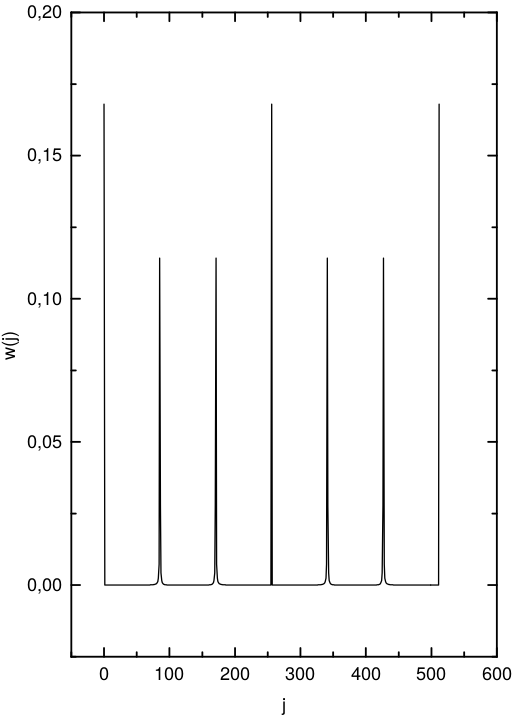
\includegraphics[width=\linewidth]{peaks.png}\newline
	\end{columns}
}

\newcommand{\Grover}[0]{Поиск в неструктурированной базе данных (Гровер)}

\frame{
	\frametitle{\Grover}
	Квантовая база состоит из $N$ $n$-кубитовых регистов.\newline
	Пусть среди них есть регистр $\ket{\omega}$, и у нас есть квантовый оракул $f(x) = (x = \omega)$.
	$$\hat{U}_{f_{\omega}}\ket{x}\ket{y} = \ket{x}\ket{y + f_{\omega}(x)}$$
	$$\hat{U}_{f_{\omega}}\ket{x}\frac{\ket{0} + \ket{1}}{\sqrt{2}} = (-1)^{f_\omega(x)}\ket{x}\frac{\ket{0} + \ket{1}}{\sqrt{2}}$$
	$$\hat{U}_\omega = 1 - 2\ket{\omega}\bra{\omega}$$
	$$\ket{s} = \frac{1}{\sqrt{N}}\sum_{x=0}^{N-1}\ket{x}$$
	$$\hat{U}_s = 2\ket{s}\bra{s} - 1,\; \hat{U}_G = \hat{U}_s\hat{U}_\omega$$
	$$\hat{U}_G^m\ket{s} = \ket{\omega};\; m = \Big[ {\frac{\pi}{4}\sqrt{N}} \Big]$$
}

\section{Проблемы}

\frame{
	\frametitle{Трудности практической реализации}
	Основная проблема - трудно изолировать квантовую частицу от внешних воздействий.\newline
	Способы продлить время жизни частицы:
	\begin{itemize}
		\item Улучшение систем хранения частиц.
		\item Реализация алгоритмов исправления ошибок.
	\end{itemize}
}

\frame{
	\frametitle{Типы ошибок}
	\begin{itemize}
		\item Инверсия бита: $\ket{0} \rightarrow \ket{1}$
		\item Ошибка фазы: $\ket{1} \rightarrow -\ket{1}$
		\item Малые ошибки: $a\ket{0} + b\ket{1} \rightarrow a'\ket{0} + b'\ket{1}$
		\item Декогеренция
	\end{itemize}
}

\frame{
	\frametitle{Алгоритм исправления ошибок}
	Можно хранить не один, а 3 кубита, и исправлять одиночную инверсию большинством голосов.
	$$a\ket{0} + b\ket{1} \rightarrow a\ket{000} + b\ket{111}$$
	$$\ket{\psi} = \hat{U}_{cnot}^{12}\hat{U}_{cnot}^{23}(a\ket{0} + b\ket{1})\ket{00} = a\ket{000} + b\ket{111}$$
	$$\hat{E} = e_0(t) + e_1(t)\sigma_x^{(1)} + e_2(t)\sigma_x^{(2)} + e_3(t)\sigma_x^{(3)}$$
	$$\hat{E}\ket{\psi} = e_0(t)(a\ket{000} + b\ket{111}) + e_1(t)(a\ket{100} + b\ket{011}) +$$
	$$+ e_2(t)(a\ket{010} + b\ket{101}) + e_3(t)(a\ket{001} + b\ket{110})$$
	$$\hat{S}\ket{x_1 x_2 x_3}\ket{0 0} = \ket{x_1 x_2 x_3}\ket{x_1 + x_2, x_2 + x_3}$$
	Измеряя состояния последих двух битов, можно узнать, какие биты инвертировать, чтобы исправить ошибку.
}

\frame{
	\frametitle{Декогеренция}
	$$\hat{\rho} = \ket{\phi}\bra{\phi} = (\alpha\ket{0} + \beta\ket{1})(\alpha^\ast\bra{0} + \beta^\ast\bra{1}) =$$
	$$= |\alpha|^2\ket{0}\bra{0} + \gc{\alpha\beta^\ast}\ket{0}\bra{1} + \gc{\beta\alpha^\ast}\ket{1}\bra{0} + |\beta|^2\ket{1}\bra{1}$$
	$$\langle\gc{\alpha^\ast\beta}\rangle = 0 \; \Rightarrow \; \hat{\rho} = |\alpha|^2\ket{0}\bra{0} + |\beta|^2\ket{1}\bra{1}$$
	При декогеренции кубит превращается в обычный бит, только плохого качества.
}

\section{Недавние достижения}

\frame{
	\frametitle{Недавние достижения}
	\pause
	2014
	\begin{itemize}
		\item Осуществена квантовая телепортация на дистанцию 3 метра без ошибок.
		\item Факторизовано на квантовом устройстве наибольшее на данный момент число --- 56153.
	\end{itemize}
	\pause
	2016
	\begin{itemize}
		\item Используя 9 кубитов, была точно просимулирована молекула водорода (Google).
	\end{itemize}
	\pause
	2017
	\begin{itemize}
		\item Сделано квантовое устройство с 2000 кубитами\newline(D-Wave 2000Q).
	\end{itemize}
}

\frame{
	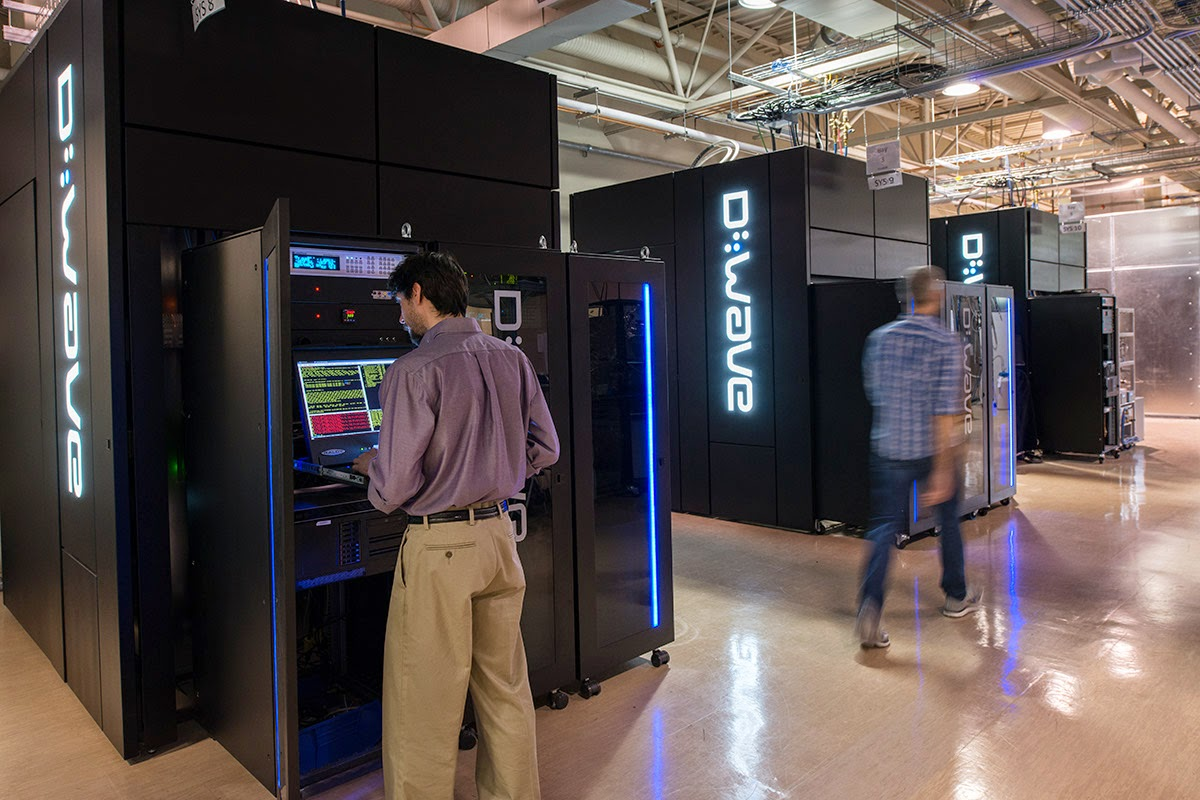
\includegraphics[width=\textwidth]{d-wave-out-01.jpg}
}

\frame{
	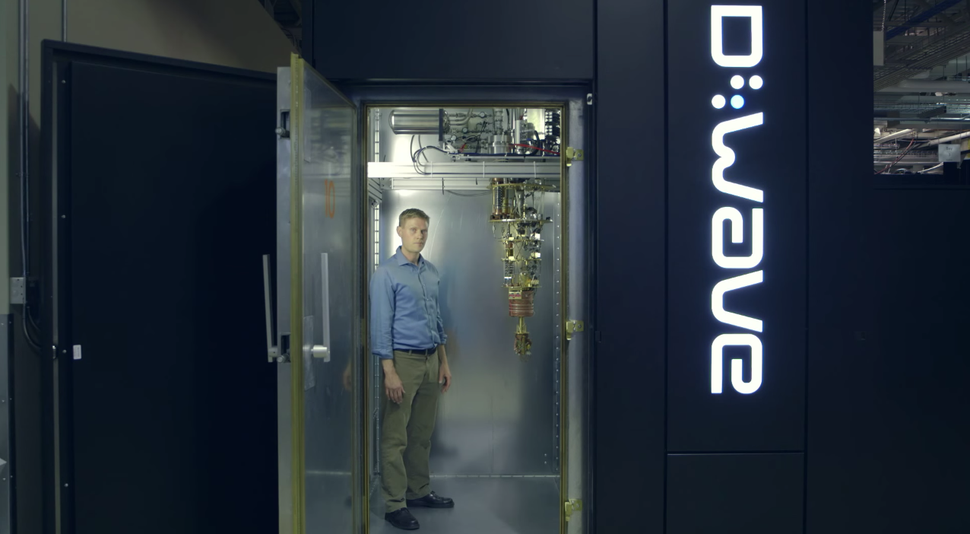
\includegraphics[width=\textwidth]{d-wave-out-02.png}
}

\setlength{\TPHorizModule}{1pt}
\setlength{\TPVertModule}{1pt}
\frame{
	\begin{textblock}{150}(0,-90)
	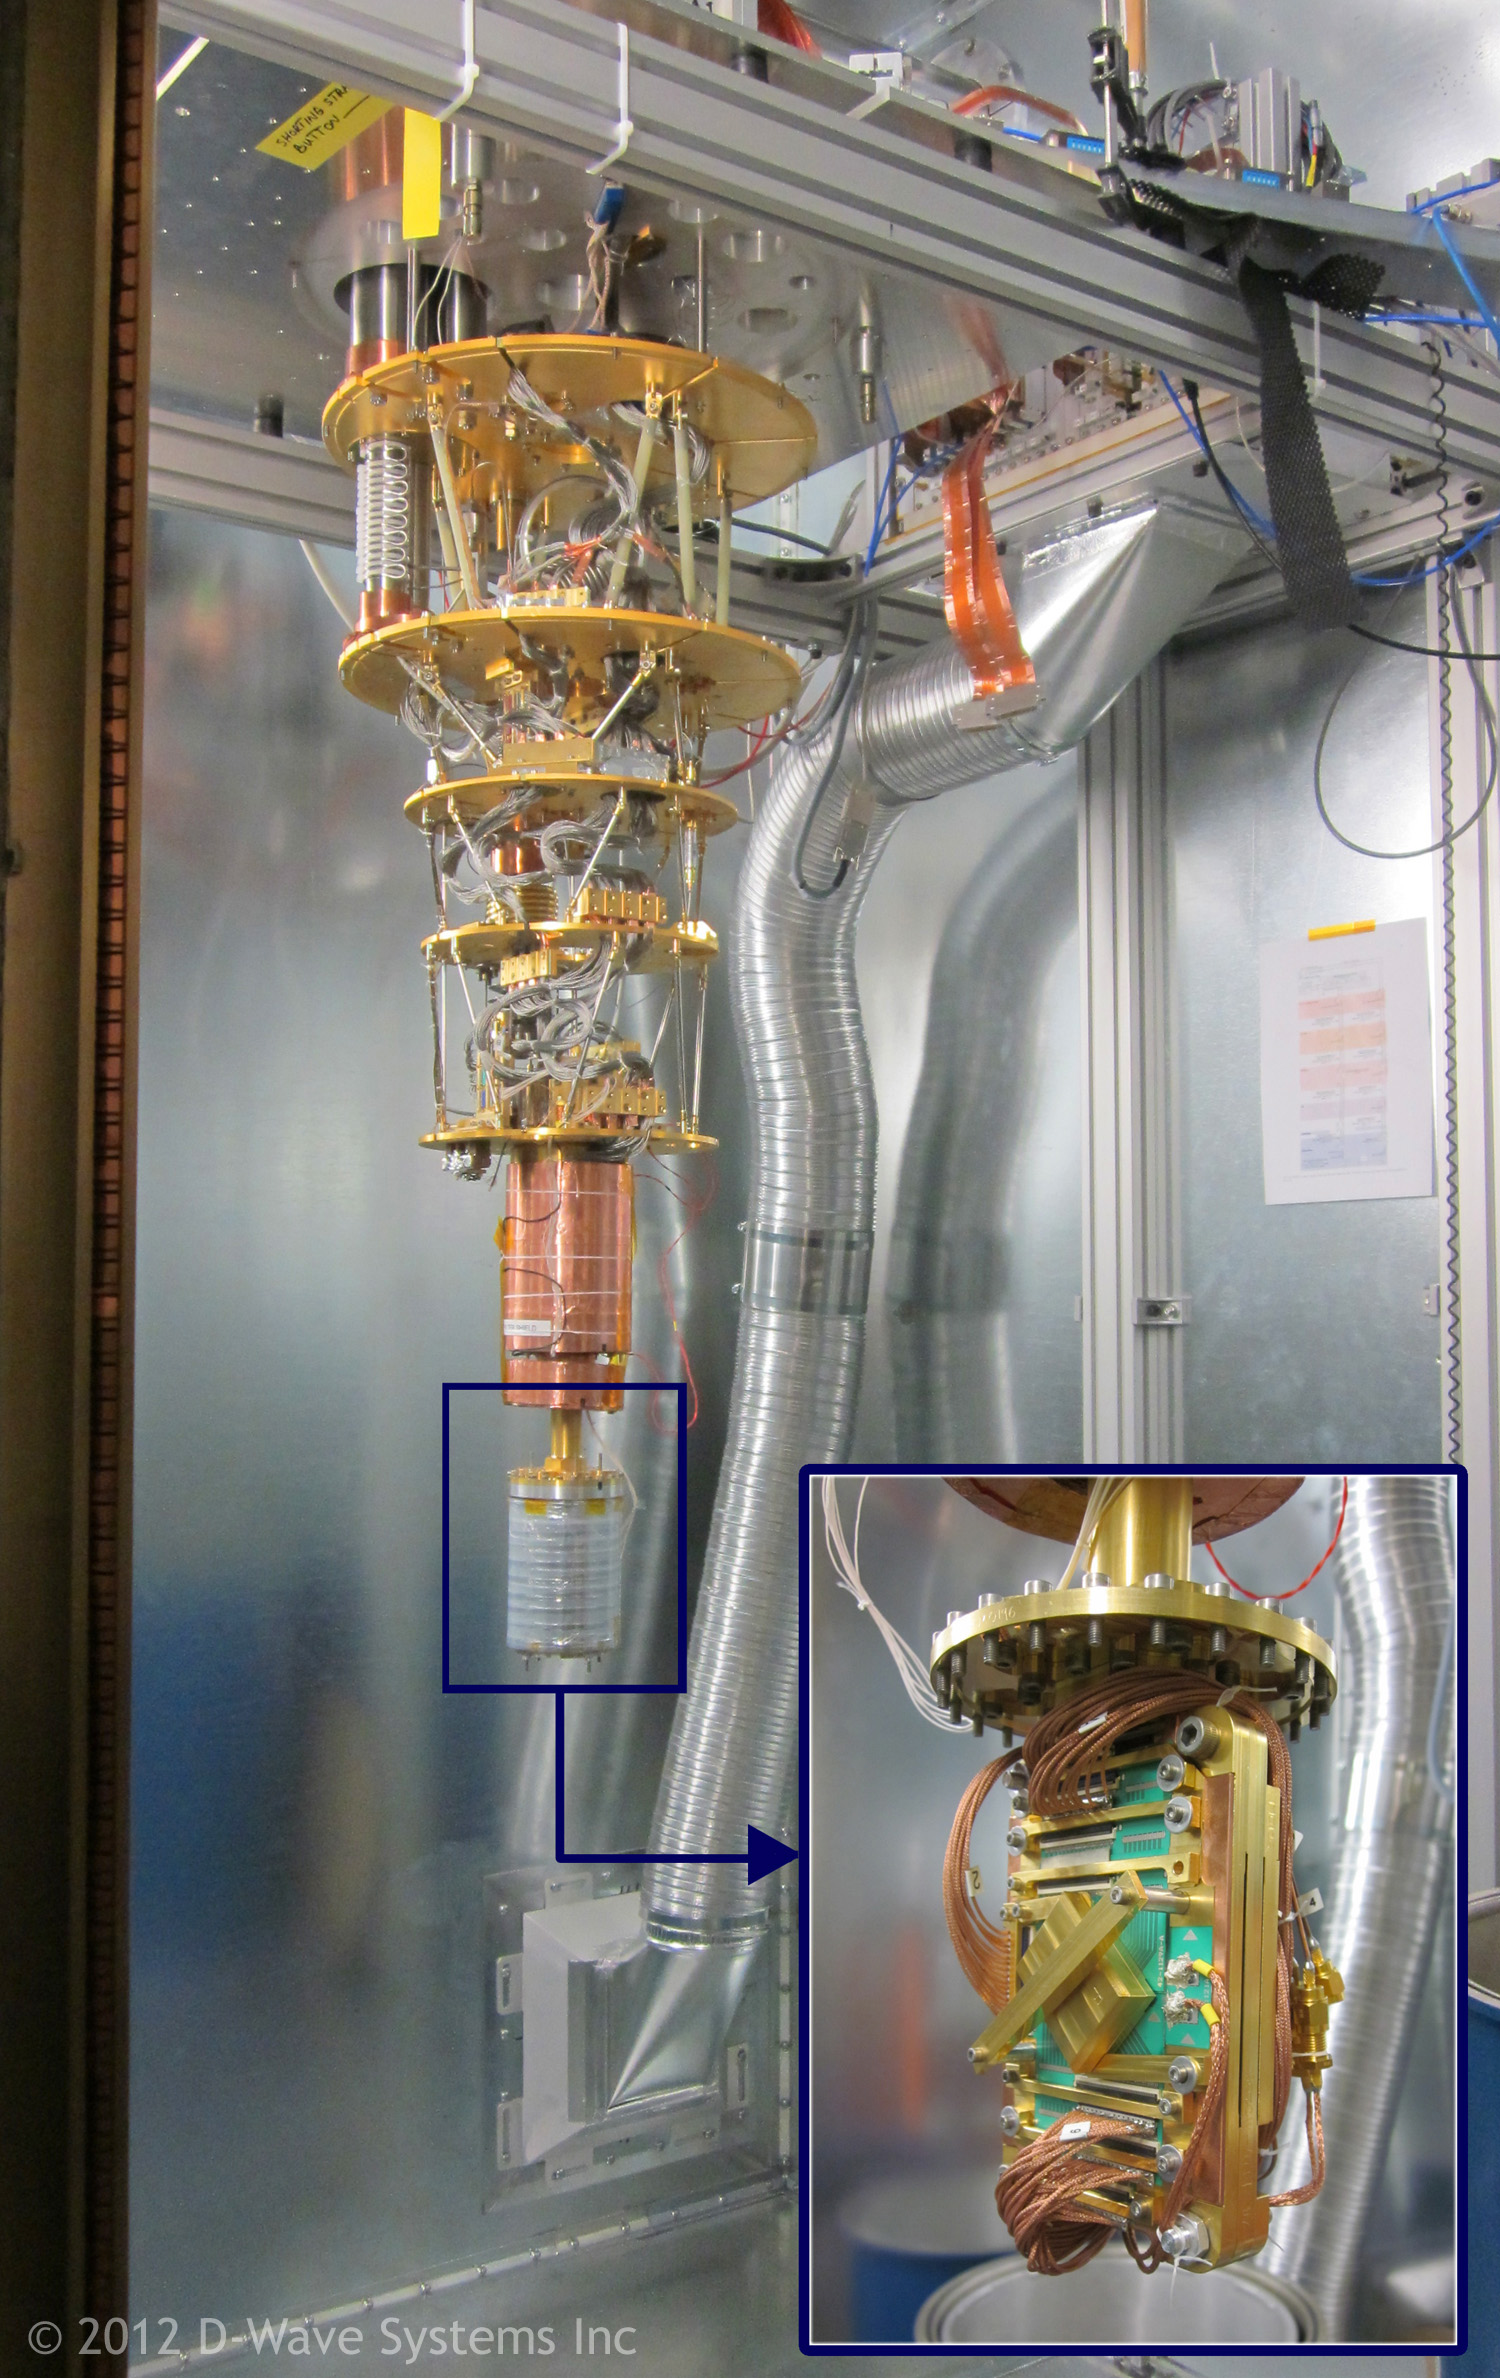
\includegraphics[width=\linewidth]{d-wave-in-01.jpg}
	\end{textblock}
	\begin{textblock}{150}(160,-90)
	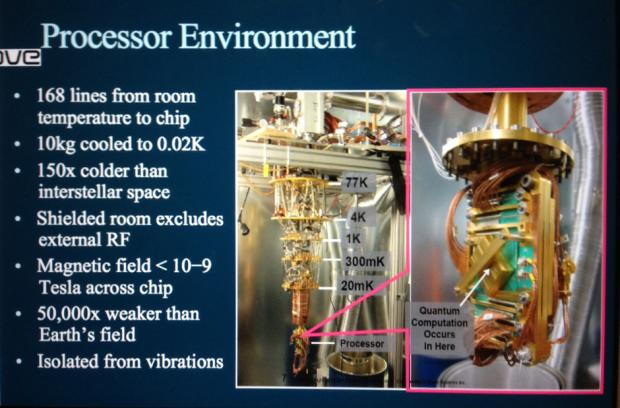
\includegraphics[width=\linewidth]{d-wave.jpg}
	\end{textblock}
	\begin{textblock}{150}(160,20)
	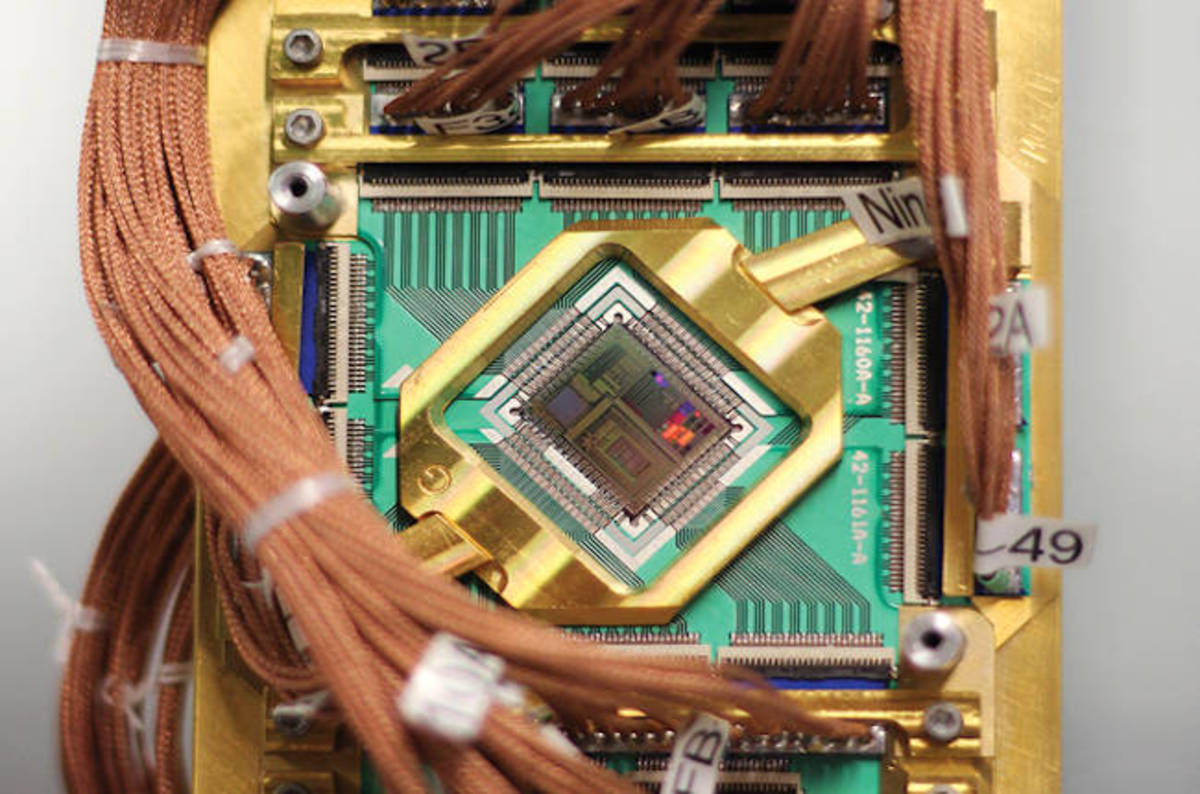
\includegraphics[width=\linewidth]{d-wave-in-02.jpg}
	\end{textblock}
}
\frame{
	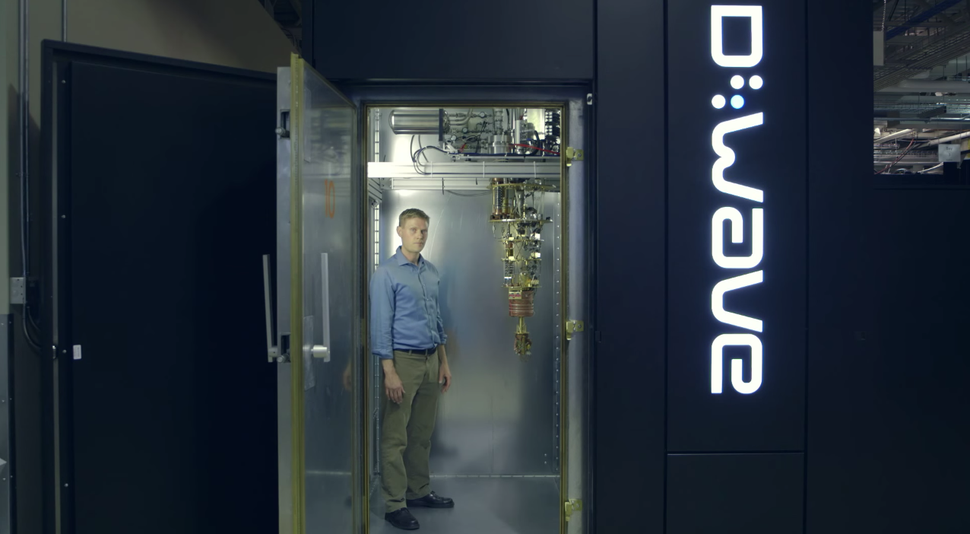
\includegraphics[width=0.5\textwidth]{d-wave-out-02.png}
}

\end{document}
